%_____________________________________________________________________________________________
% LATEX Template: Department of Comp/IT BTech Project Reports
% Sample Chapter
% Sun Mar 27 10:25:35 IST 2011
%
% Note: Itemization, enumeration and other things not shown. A sample figure is included.
%_____________________________________________________________________________________________

\chapter{Introduction}
Computer vision is a field of computer science that works on enabling computers to see, identify and process images in the same way that human vision does, and then provide appropriate output. It is like imparting human intelligence and instincts to a computer. In reality though, it is a difficult task to enable computers to recognize images of different objects.
Computer vision is closely linked with artificial intelligence, as the computer must interpret what it sees, and then perform appropriate analysis or act accordingly. With the help of computer vision and deep learning the process of website development can be aided to make it more robust,flexible and fast.

\section{The gap between design and development}
%Th is is a section. We can cite a reference like this: \cite{INTERNET} Citation. See references.tex for the entry.
With the technological advancement in the 21st-century, everybody wants to experience the best technology without spending too much of their time and exhausting their busy brains. The same goes for surfing the websites or mobile applications as well where the quick and efficient the website or the mobile application responds, the successful outcomes it obtains. In short, it is about consumers nowadays! And, when it comes to the mobile application or website user satisfaction, most technology firms turn towards the applications’ User Interface (UI) and User Experience Design (UX).
The User Interface (UI), is the process of improving the presentation and the interactivity of the web or mobile application. It focuses on the app’s look and interacts with the users. Each screen, page, buttons and other visual elements you see while using an application is the User Interface of that application.
User Interface Design process involves a lot a creativity that starts on a whiteboard where designers share ideas. Once a design is drawn, and after iterations among the design team, a design mockup is ready. Now, these mockups are passed on to the Development Team. The developers work on to convert these mockups into actual functional units. This is again verified by the design team and a final product is ready after many iterations.
Work stops whenever one discipline finishes a portion of the project and passes responsibility to another discipline. This process takes several iterations and consumes a lot of effort and time. There is a big gap in how the ideas are exchanged between designers and developers. There are ways in which the designer designs an expected view with various drawing tools like Photoshop and CorelDraw. Developers try to mimic these prototypes. But the output of drawing tools is of no help in terms of generating the code for the developer. This shows there is a gap in this process and a big scope of improvement in the whole process of development.

\section{Bridging the gap}
There are various options being tried to bridge the gap. There are drawing software like PhotoShop, CorelDraw which are used by designers to generate the actual design mockups. So that the Development team can try and mimic the exact design submitted by the Design team. But efforts are consumed on both the design side to create the mockups and the development side to mimic them. The purpose of mockups is just to transfer the ideas.
What if we can automate this whole process and try to bridge the gap. An application that takes the photographs of the whiteboard drawings of the Design Team and gives a functional editable code for the developer to work on. This will save time on both ends by removing the idea of creating design mockups on specialised software and developers trying to mimic it.

\section{Role of Computer Vision and ML}
Computer Vision enables developer to leverage existing ‘machine capabilities’ to sense patterns and shapes.the
Computer Vision forms the core of this service. Neural Networks based architectures, such as R-CNN, Fast-RCNN or YOLO built on standard ML libraries like TensorFlow and Keras will help to detect the DOM components user wants in the web page. Detecting DOM elements, unlike common objects, is a comparatively difficult objective; mainly because of the lack of the necessary amount of training data.

	\subsection{Neural Networks}
	Artificial Neural Networks are the biologically inspired simulations performed on the computer to perform certain specific tasks like clustering, classification, pattern recognition etc. Artificial Neural Networks, in general — is a biologically inspired network of artificial neurons configured to perform specific tasks. Neural networks resemble the human brain in the following two ways -

	\begin{itemize}
		\item A neural network acquires knowledge through learning.
		\item A neural network’s knowledge is stored within inter-neuron connection strengths known as synaptic weights.
	\end{itemize}

	\begin{figure}[H]
		\centering
		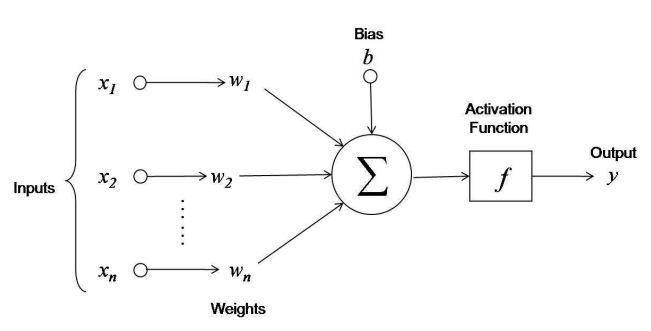
\includegraphics[width=6in]{artificial_neuron}
		\caption
		{Basic structure of an artificial neuron}
	\end{figure}

	Artificial neural networks can be viewed as weighted directed graphs in which artificial neurons are nodes and directed edges with weights are connections between neuron outputs and neuron inputs. The Artificial Neural Network receives input from the external world in the form of pattern and image in vector form. These inputs are mathematically designated by the notation x(n) for n number of inputs. Each input is multiplied by its corresponding weights. Weights are the information used by the neural network to solve a problem. Typically weight represents the strength of the interconnection between neurons inside the neural network.

	\begin{figure}[H]
		\centering
		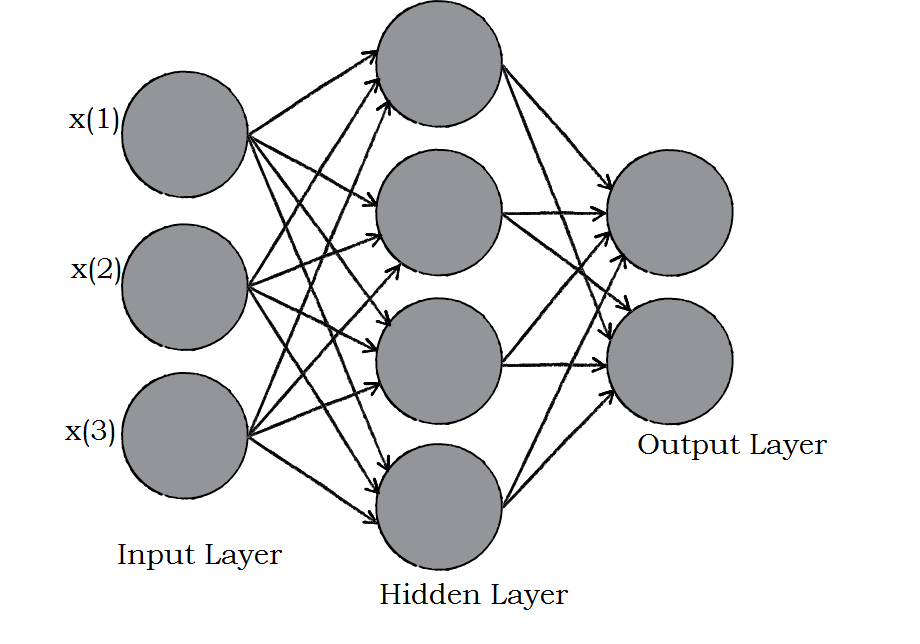
\includegraphics[width=6in]{multilayer_nn}
		\caption
		{Multilayer Neural Network with a hidden layer}
	\end{figure}

	The weighted inputs are all summed up inside computing unit (artificial neuron). In case the weighted sum is zero, bias is added to make the output not- zero or to scale up the system response. Bias has the weight and input always equal to ‘1’. The sum corresponds to any numerical value ranging from 0 to infinity. In order to limit the response to arrive at desired value, the threshold value is set up. For this, the sum is passed through activation function. The activation function is set of the transfer function used to get desired output. There are linear as well as the nonlinear activation function.

	\subsection{Convolutional Neural Network}

	The image is divided into receptive fields that feed into a convolutional layer, which then extracts features from the input image. The next step is pooling, which reduces the dimensionality of the extracted features (through down-sampling) while retaining the most important information (typically through max pooling).
	Another convolution and pooling step is then performed that feeds into a fully connected multilayer perceptron. The final output layer of this network is a set of nodes that identify features of the image (in this case, a node per identified number). You train the network by using back-propagation

	\begin{figure}
		\centering
		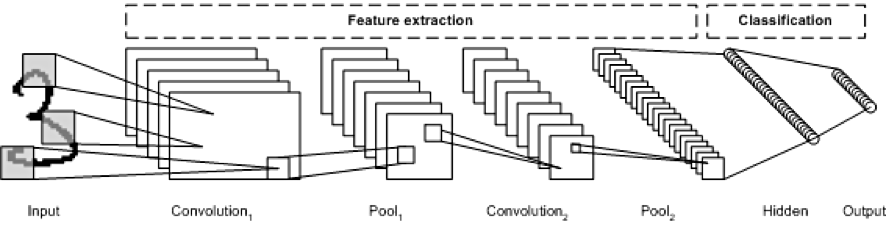
\includegraphics[width=6in]{cnn}
		\caption
		{A Convolutional neural network consisting of multiple steps}
	\end{figure}

	\subsection{RCNN}

	For each image, there is a sliding window to search every position within the image as below. It is a simple solution. However, different objects or even same kind of objects can have different aspect ratios and sizes depending on the object size and distance from the camera. And different image sizes also affect the effective window size. This process will be extremely slow if we use deep learning CNN for image classification at each location.
	In R-CNN the CNN is forced to focus on a single region at a time because that way interference is minimized because it is expected that only a single object of interest will dominate in a given region. The regions in the R-CNN are detected by selective search algorithm followed by resizing so that the regions are of equal size before they are fed to a CNN for classification and bounding box regression.
	Steps:

	\begin{itemize}
		\item NN uses selective search to generate about 2K region proposals, i.e. bounding boxes for image classification.
		\item Then, for each bounding box, image classification is done through CNN.
		\item Finally, each bounding box can be refined using regression.
	\end{itemize}

	\subsection{YOLO (You Only Look Once)}

	Compared to other region proposal classification networks (fast RCNN) which perform detection on various region proposals and thus end up performing prediction multiple times for various regions in a image, Yolo architecture is more like FCNN (fully convolutional neural network) and passes the image (nxn) once through the FCNN and output is (mxm) prediction. This the architecture is splitting the input image in mxm grid and for each grid generation 2 bounding boxes and class probabilities for those bounding boxes. Note that bounding box is more likely to be larger than the grid itself.
	It also makes predictions with a single network evaluation unlike systems like R-CNN which require thousands for a single image. This makes it extremely fast, more than 1000x faster than R-CNN and 100x faster than Fast R-CNN

	\subsection{Optical Character Recognition}

	OCR (optical character recognition) is the recognition of printed or written text characters by a computer. This involves photo scanning of the text character-by-character, analysis of the scanned-in image, and then translation of the character image into character codes, such as ASCII, commonly used in data processing. The current age OCR implementations work with a very superior accuracy for printed english text but the accuracies are lower for handwritten english text. Advancements in OCR have enabled detection of not only printed text but also handwritten content. Multiple cloud services provide APIs for recognition of english handwritten text.


%_____________________________________________________________________________________________
